\chapter{\msyh 信息收集}
\begin{center}
\kai
题目:《柳》\par
作者:寇准(961-1023)\par
晓带轻烟间杏花,晚凝深翠拂平沙。\par
长条别有风流处,密映钱塘苏小家。 \par

\end{center}

\fzsk 
\section{\msyh  信息收集}

如何收集puppet执行后的信息呢? 我这里是采用的foreman来收集puppet执行情况以及服务器上的facter配置信息。通常,在c/s方式部署puppet的时候,puppet agent执行的结果反馈给puppet master, 然后由puppet master统计提交给foreman或者puppet dashboard。在这里,因为没有puppet master,所以我们需要直接把puppet执行后情况发送给foreman。思路是在puppet agent的puppet.conf配置文件里面加上log report功能,然后自定义一个foreman的log report方法。

\codefont\tiny \begin{lstlisting}
[main]
report = true
reports = foreman

\end{lstlisting}

\fzsk\normalsize

然后再创建一个/var/lib/puppet/lib/puppet/reports/foreman.rb的文件,内容如下:

\codefont\tiny \begin{lstlisting}

# <%= ERB.new(File.read(File.expand_path("_header.erb",File.dirname(file)))).result(binding) -%>
# copy this file to your report dir - e.g. /usr/lib/ruby/1.8/puppet/reports/
# add this report in your puppetmaster reports - e.g, in your puppet.conf add:
# reports=log, foreman # (or any other reports you want)

# URL of your Foreman installation
$foreman_url='http://foremanserver:8000'
# if CA is specified, remote Foreman host will be verified
#$foreman_ssl_ca = "<%= @ssl_ca -%>"
# ssl_cert and key are required if require_ssl_puppetmasters is enabled in Foreman
#$foreman_ssl_cert = "<%= @ssl_cert -%>"
#$foreman_ssl_key = "<%= @ssl_key -%>"

require 'puppet'
require 'net/http'
require 'net/https'
require 'uri'

Puppet::Reports.register_report(:foreman) do
    Puppet.settings.use(:reporting)
    desc "Sends reports directly to Foreman"

    def process
      begin
        uri = URI.parse($foreman_url)
        http = Net::HTTP.new(uri.host, uri.port)
        http.use_ssl     = uri.scheme == 'https'
        if http.use_ssl?
          if $foreman_ssl_ca && !$foreman_ssl_ca.empty?
            http.ca_file = $foreman_ssl_ca
            http.verify_mode = OpenSSL::SSL::VERIFY_PEER
          else
            http.verify_mode = OpenSSL::SSL::VERIFY_NONE
          end
          if $foreman_ssl_cert && !$foreman_ssl_cert.empty? && $foreman_ssl_key && !$foreman_ssl_key.empty?
            http.cert = OpenSSL::X509::Certificate.new(File.read($foreman_ssl_cert))
            http.key  = OpenSSL::PKey::RSA.new(File.read($foreman_ssl_key), nil)
          end
        end
        req = Net::HTTP::Post.new("#{uri.path}/reports/create?format=yml")
        req.set_form_data({'report' => to_yaml})
        response = http.request(req)
      rescue Exception => e
        raise Puppet::Error, "Could not send report to Foreman at #{$foreman_url}/reports/create?format=yml: #{e}"
      end
    end
end

\end{lstlisting}
\fzsk\normalsize

这个脚本会把puppet执行日志发送给foreman。这样就可以知道puppet执行情况。
\begin{center}

\includegraphics[width=0.6\textwidth]{1.png}
\end{center}
\par
另外还有一个数据的收集,那就是facter收集的数据,便于做资产统计,比如统计服务器序列号,软件的版本号,网卡的速率等。下面这个脚本,会把/var/lib/puppet/yaml/facts/hostname.yaml文件内的内容,推送到foreman里面的fact值里面。
\codefont\tiny \begin{lstlisting}
#! /usr/bin/env ruby
#
# This scripts runs on remote puppetmasters that you wish to import their nodes facts into Foreman
# it uploads all of the new facts its encounter based on a control file which is stored in /tmp directory.
# This script can run in cron, e.g. once every minute
# if you run it on many puppetmasters at the same time, you might consider adding something like:
# sleep rand(10) # that not all PM hammers the DB at once.
# ohadlevy@gmail.com

# puppet config dir
puppetdir="/var/lib/puppet"

# URL where Foreman lives
url="http://youip:8000"

# Temp file keeping the last run time
stat_file = "/tmp/foreman_fact_importer"

require 'fileutils'
require 'net/http'
require 'net/https'
require 'uri'

last_run = File.exists?(stat_file) ? File.stat(stat_file).mtime.utc : Time.now - 365*60*60

Dir["#{puppetdir}/yaml/facts/*.yaml"].each do |filename|
  last_fact = File.stat(filename).mtime.utc
  if last_fact > last_run
    fact = File.read(filename)
    puts "Importing #{filename}"
    begin
      uri = URI.parse(url)
      http = Net::HTTP.new(uri.host, uri.port)
      if uri.scheme == 'https' then
        http.use_ssl = true
        http.verify_mode = OpenSSL::SSL::VERIFY_NONE
      end
      req = Net::HTTP::Post.new("/fact_values/create?format=yml")
      req.set_form_data({'facts' => fact})
      response = http.request(req)
    rescue Exception => e
      raise "Could not send facts to Foreman: #{e}"
    end
  end
end
FileUtils.touch stat_file

\end{lstlisting}
\fzsk\normalsize
现在,有趣的的问题来了,/var/lib/puppet/yaml/facts/hostname.yaml 文件怎么创建呢,c/s模式里面,是puppetmaster负责的。这里,我们直接用facter  -y 命令来产生这个文件。这还产生了一个另外好处,不用自定义facter的脚本,就能收集任何fact值,比如我要收集一个软件版本的信息,我直接用shell脚本取软件版本号,然后用echo把信息追加到yaml文件里面。下面这个脚本我用来生成yaml文件。并且收集了几个软件的版本和网卡的速率。

\codefont\tiny \begin{lstlisting}
#!/bin/bash
cf=/var/lib/puppet/yaml/facts/`hostname`.yaml
mkdir -p /var/lib/puppet/yaml/facts
facter -y  > $cf
sed -i '/ppp/d' $cf

m2v=$(dpkg -l|grep mycomp-l2tpns|awk '{print $3}')
m3v=$(dpkg -l|grep mycomp-openvpn|awk '{print $3}')
m2id=$(grep "id=" /opt/mycomp/l2tpns/etc/vppp.conf |sed 's/id=//')
echo "  m2ver: ${m2v:-NULL}" >>$cf
echo "  m3ver: ${m3v:-NULL}" >>$cf
echo "  m2id: ${m2id:-NULL}" >>$cf


mii-tool 2>/dev/null |sed 's/^/  mii/' >>$cf
/usr/local/bin/push-fact.ruby


\end{lstlisting}
\fzsk\normalsize

\begin{center}
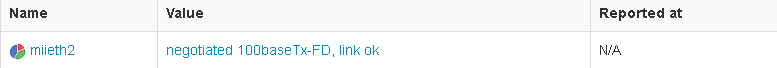
\includegraphics[width=0.6\textwidth]{2.png}
\end{center}
这个脚本会在每次执行完puppet以后调用。把需要收集的fact值发到foreman。

\par

如果你思路还清晰的话,应该记的,每次都是从crontab执行脚本来下载puppet代码执行,这个脚本最后一行会执行/bin/run-parts /etc/puppet/file/shell/autorun/; 会把 /etc/puppet/file/shell/autorun/目录下的所有脚本执行一次。有个好处,避免每次用exec资源来执行脚本。同时我还可以加一个/etc/puppet/file/shell/perhost/目录,目录下面按主机名建目录,里面放上特定的机器需要执行的特定代码。只需要再加一句行/bin/run-parts /etc/puppet/file/shell/perhost/`hostname`/

\par
利用autorun和perhost目录,可以灵活的做一些批量任务,而不用去修改puppet代码,写exec资源等。


